
%\DeclareMathOperator{\tri}{tri} \DeclareMathOperator{\rect}{rect}
%\DeclareMathOperator{\sgn}{sgn} \DeclareMathOperator{\ramp}{ramp}
%\DeclareMathOperator{\sinc}{sinc}


\subsection{Cyclometrische functies}
%\begin{itemize}
%\item Wat zijn de cyclometrische functies?
%\item Waarom zijn de cyclometrische functies eigenlijk geen functies (maar
%slechts relaties)?
%\item Wat zijn de grafieken van Arcsin, Arccos, Arctan en Arccot?
%\end{itemize}

\subsubsection{Relatie versus functie}

Wanneer we van een (in radialen gemeten) hoek $x$ weten dat $\sin x=\frac{1}{2}$,
dan zijn er voor $x$ oneindig veel mogelijkheden. De sinus is namelijk
een periodieke functie, en bovendien wordt elke waarde (behalve 1
en -1) gedurende /'e/'en periode twee maal aangenomen. Zo geldt $\sin x=\frac{1}{2}$
voor $x=\frac{\pi}{6}$ en voor $x=\frac{5\pi}{6}$, en bij elk van
die hoeken kunnen we nog willekeurige gehele veelvouden van $2\pi$
optellen. Als je je nu zou afvragen welke $x$-waarde levert voor
de sinusfunctie $\frac{1}{2}$ op, dan zou je moeten antwoorden met
$x=\ldots,\frac{\pi}{6},\frac{5\pi}{6},\frac{\pi}{6}+2\pi,\ldots$
En dat is nu niet bepaald duidelijk.

\medskip{}


\noindent We defini/"eren de cyclometrische functies (ook wel arcfuncties
of boogfuncties) als de inverse functies van de goniometrische functies.
Maar, zoals we net gezien hebben, is de inverse van de goniometrische
functie in feite geen functie maar gewoon een \emph{relatie}. In een
relatie horen bij /'e/'en waarde uit het domein ($x$-waarde) meerdere
(tot zelfs oneindig) veel beelden ($y$-waarden). Om tot een functie
te komen moeten we het domein van de oorspronkelijk functie beperken
(hier was dit de sinus functie). Dit beperkt domein noemen we een
hoofdwaarde-interval.

\medskip{}


\noindent De cyclometrische functie wordt met een hoofdletter geschreven
(bijv: $\textrm{Arcsin}$)

\noindent De cyclometrische relatie wordt met een kleine letter geschreven
(bijv: $\arcsin$)

\medskip{}


\noindent De vergelijking $y=\arcsin(x)$ is geen functie, want met
elke $x$-waarde komen oneindig veel $y$-waarden overeen. \medskip{}


\noindent Zo voldoet $y=...,\:\frac{\pi}{6}\:(30{^\circ}),\:\frac{5\pi}{6}\:(150{^\circ}),\:\frac{13\pi}{6}\:(390{^\circ}),...$
aan $y=\arcsin(\frac{1}{2})$

\medskip{}


\noindent Om tot een functie te komen zullen we het domein van $y=\sin(x)$
beperken. We kiezen als hoofdwaarde-interval voor $[-\frac{\pi}{2},\frac{\pi}{2}]$.
En we noteren nu de inverse functie van de sinusfunctie als $y=\textrm{Arcsin}(x)$

\noindent Nu geldt: $\textrm{Arcsin}(\frac{1}{2})=\frac{\pi}{6}\:(30\text{\textdegree})$

\medskip{}


Voor de cosinus, tangens en cotangens, waarbij soortgelijke problemen
spelen, heeft men eveneens zulke voorkeursintervallen afgesproken:
$[0,\pi]$ voor de cosinus en $]-\frac{\pi}{2},\frac{\pi}{2}[$ voor
de tangens. Aangezien $\tan(\frac{\pi}{2})$ oneindig is, is de tangens
niet gedefini/"eerd voor hoeken gelijk aan $\frac{\pi}{2}$ en $-\frac{\pi}{2}$,
vandaar de notatie met open i.p.v. gesloten haakjes.

\medskip{}


\noindent Opmerking: op je rekenmachine vind je de cyclometrische
functies meestal terug onder de namen (toetsen) ${\displaystyle \sin^{-1}}$,
${\displaystyle \cos^{-1}}$ en ${\displaystyle \tan^{-1}}$. Verwar
dit niet met ${\displaystyle \frac{1}{\sin x}=\left(\sin x\right)^{-1}}$!!

\noindent In tekstboeken vind je ook de notatie $\textrm{bgsin}(x)$
of $\textrm{argsin}(x)$ voor $\textrm{arcsin}(x)$ en $\textrm{Bgsin}(x)$
of $\textrm{Argsin}(x)$ voor $\textrm{Arcsin}(x)$. Hierbij staan
de letter ``bg'' voor boog en ``arg'' voor argument.


\subsubsection{De cyclometrische functies}

De grafieken van deze functies worden bekomen door spiegeling ten
opzichte van de rechte $y=x$ van een gepaste beperking van de grafiek
van de overeenkomstige goniometrische functies.

\begin{itemize}
\item{De inverse van de sinusfunctie}

\noindent $y=\textrm{Arcsin}(x)$ met ${\displaystyle y\in[-\frac{\pi}{2},\frac{\pi}{2}]}$

De inverse van de sinusfunctie $y=\textrm{Arcsin}(x)$ kan je enkel
voor ${\displaystyle x\in[-1,1]}$ berekenen.

De inverse van de sinusfunctie ligt altijd tussen ${\displaystyle y\in[-\frac{\pi}{2},\frac{\pi}{2}]}$.

\begin{figure}
	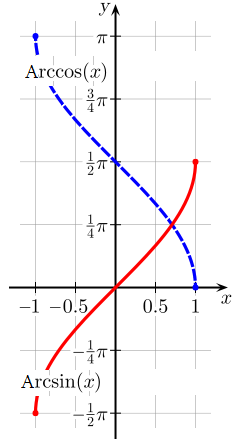
\includegraphics{2_elem_rekenvaardigheden_B/inputs/Arcsine_Arccosine_svg}
\end{figure}



\item{De inverse van de cosinusfunctie}

\noindent $y=\textrm{Arccos}(x)$ met ${\displaystyle y\in[0,\pi]}$

De inverse van de cosinusfunctie $y=\textrm{Arccos}(x)$ kan je enkel
voor ${\displaystyle x\in[-1,1]}$ berekenen.

De inverse van de cosinusfunctie ligt altijd tussen ${\displaystyle y\in[0,\pi]}$.


\item{De inverse van de tangensfunctie}

\noindent $y=\textrm{Arctan}(x)$ met ${\displaystyle y\in]-\frac{\pi}{2},\frac{\pi}{2}[}$

De inverse van de tangensfunctie $y=\textrm{Arctan}(x)$ kan je voor
alle ${\displaystyle x}$ berekenen.

De inverse van de tangensfunctie ligt altijd tussen ${\displaystyle y\in]-\frac{\pi}{2},\frac{\pi}{2}[}$.

De grafiek toont twee horizontale asymptoten: de lijnen $y=-\frac{\pi}{2}$
en $y=\frac{\pi}{2}$.

We noteren ook: ${\displaystyle \lim_{x\to-\infty}}\textrm{Arctan}(x)=-\frac{\pi}{2}$
en ${\displaystyle \lim_{x\to+\infty}}\textrm{Arctan}(x)=\frac{\pi}{2}$.

\begin{figure}
	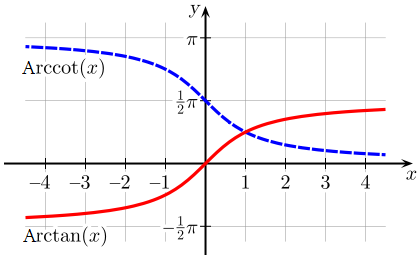
\includegraphics{2_elem_rekenvaardigheden_B/inputs/Arctangent_Arccotangent_svg}
\end{figure}



\item{De inverse van de cotangensfunctie}

\noindent $y=\textrm{Arccot}(x)$ met ${\displaystyle y\in]0,\pi[}$

De inverse van de cotangensfunctie $y=\textrm{Arccot}(x)$ kan je
voor alle ${\displaystyle x}$ berekenen.

De inverse van de cotangensfunctie ligt altijd tussen ${\displaystyle y\in]0,\pi[}$.

De grafiek toont twee horizontale asymptoten: de lijnen $y=0$ en
$y=\pi$.

We noteren ook: ${\displaystyle \lim_{x\to-\infty}}\textrm{Arccot}(x)=0$
en ${\displaystyle \lim_{x\to+\infty}}\textrm{Arccot}(x)=\pi$.

\end{itemize}

\subsubsection{Rekenregels}

Past men op een cyclometrische functie de overeenkomstige goniometrische
functie toe, dan bekomt men als resultaat het argument waarvan men
is uitgegaan.

$\begin{array}{ccc}
{\displaystyle \sin\left(\textrm{Arcsin}(x)\right)} & = & x\\
{\displaystyle \cos\left(\textrm{Arccos}(x)\right)} & = & x\\
{\displaystyle \tan\left(\textrm{Arctan}(x)\right)} & = & x\\
{\displaystyle \textrm{cot}\left(\textrm{Arccot}(x)\right)} & = & x
\end{array}$

\medskip{}


\noindent Past men in een goniometrische functie de overeenkomstige
cyclometrische functie toe, dan bekomt men als resultaat \emph{niet
noodzakelijk} het argument waarvan men is uitgegaan, maar wel een
waarde van het overeenkomstig hoofdwaarde-interval.
